% ------------------------------------------------------------------------------
% 7.3. DISEÑO DE DATOS
% ------------------------------------------------------------------------------
\subsection{7.3. Diseño de Datos}\label{sec:cap7_diseno_datos}

El diseño de datos traduce las clases persistentes del diagrama de clases (sección~\ref{sec:cap7_diagrama_clase}) a un modelo relacional implementado en PostgreSQL. El modelo consta de 32 tablas agrupadas según los seis paquetes del análisis: Cuentas y acceso (5), Convocatoria y postulación (9), Preselección con IA (4), Auditoría y adjudicación (8), Becados y asistencia (5) y Reportes y trazabilidad (1). Los nombres de tablas y columnas se escriben en minúsculas, en singular y separados por guion bajo; cada tabla tiene una clave primaria interna \textit{id} y las claves foráneas se nombran \textit{\textless{}tabla\textgreater{}\_id}.

Todas las tablas incorporan cuatro columnas comunes: \textit{codigo\_\textless{}tabla\textgreater{}}, un identificador público UUID versión 7, único y no nulo, que es el único identificador que se expone a la API y a los clientes web y móvil; \textit{creado\_en} y \textit{actualizado\_en}, que registran la fecha y hora de creación y de la última modificación; y \textit{eliminado\_en}, que implementa el borrado lógico, de modo que ningún registro se elimina físicamente. Las contraseñas se almacenan únicamente como hash (BCrypt) y los tokens de renovación de sesión y de recuperación de contraseña solo como hash (SHA-256), y los archivos se guardan en MinIO, del que la base de datos solo conserva la ruta.

\subsubsection{7.3.1. Diseño de Datos Lógico}\label{sec:cap7_datos_logico}

\paragraph{7.3.1.1. Diseño lógico de la Base de Datos.}\label{sec:cap7_logico_bd}
El diseño lógico de la base de datos representa cada tabla con sus columnas, tipos de datos, claves primarias (PK), claves foráneas (FK) y restricciones de unicidad (UQ), así como las relaciones y cardinalidades entre las tablas. La Figura~\ref{fig:diseno_logico_bd} presenta el diagrama del diseño lógico.

\begin{figure}[H]
\caption{Diseño lógico de la base de datos}
\label{fig:diseno_logico_bd}
\centering
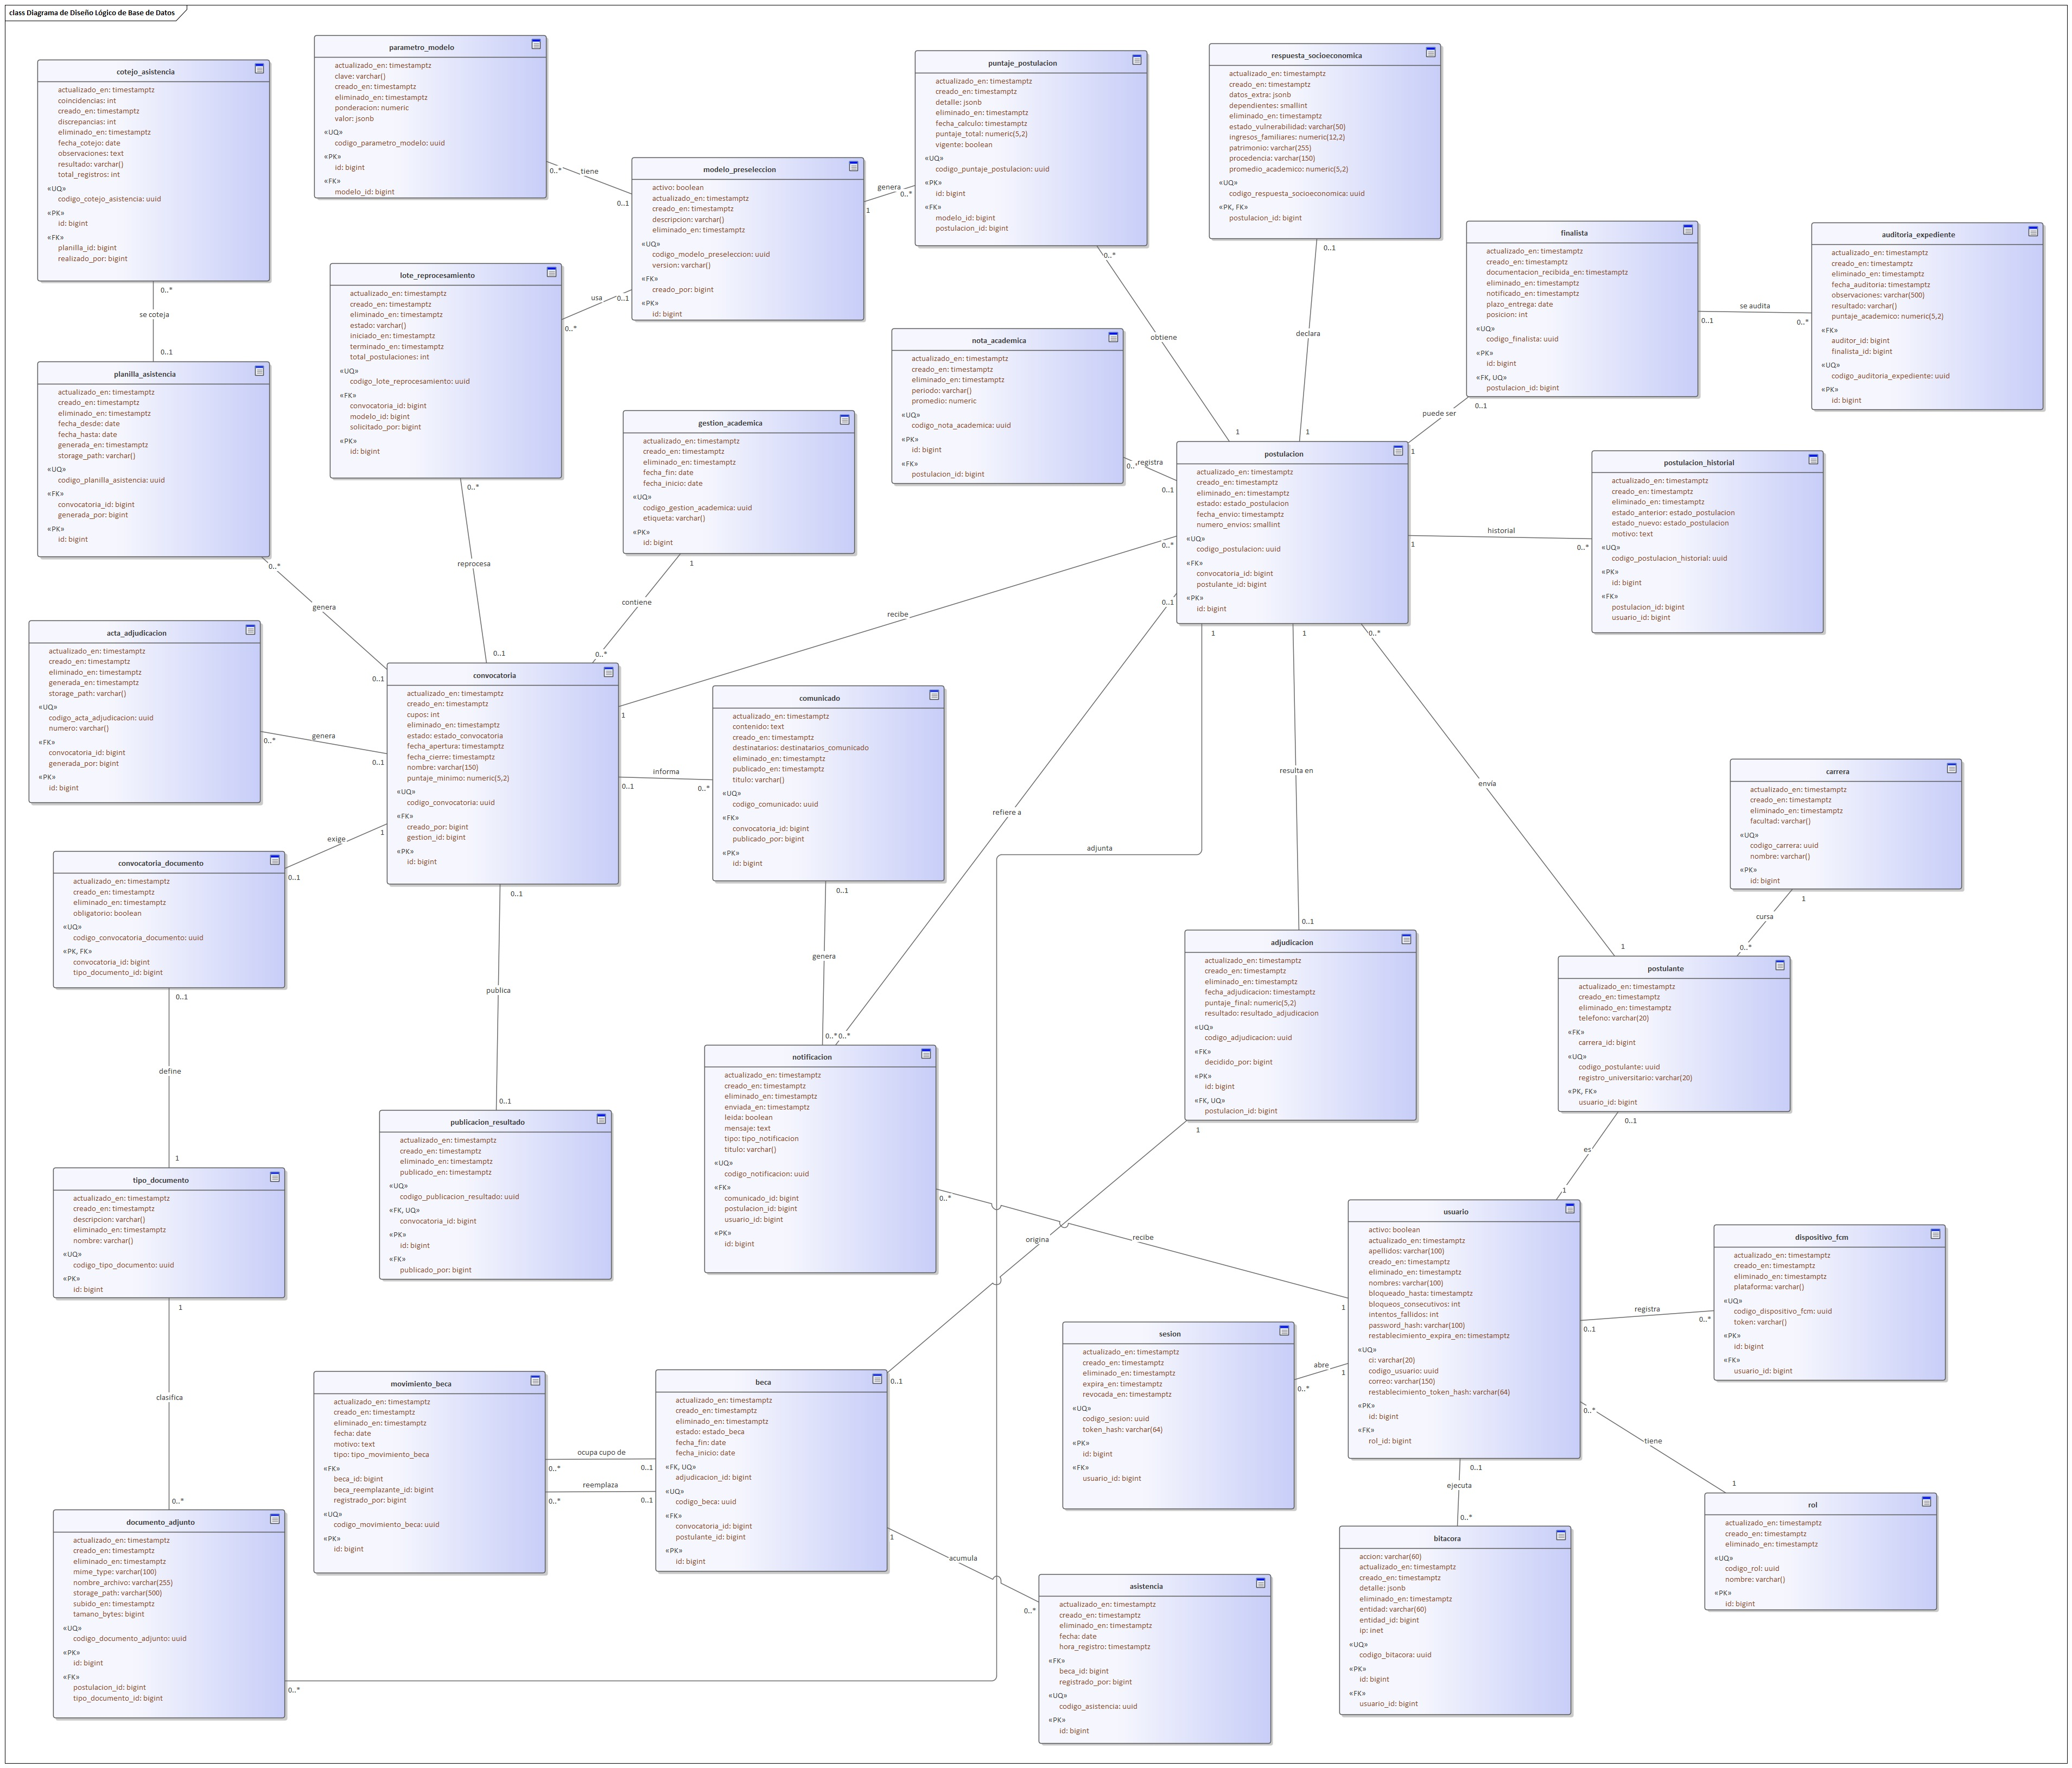
\includegraphics[width=\textwidth,height=0.8\textheight,keepaspectratio]{images/091_Diseno_Logico_Base_de_Datos.jpg}

\smallskip
\noindent\raggedright\textit{Nota.} Elaboración propia.
\end{figure}


